% vim: tw=80

\chapter{Conclusion}

For the first time, a measurement of triple-differential dijet cross sections at
has been accomplished at the LHC. The measurement has been performed using the
CMS detector at a center-of-mass energy of \SI{8}{\TeV} using the complete data
set collected in 2012 comprising \SI{19.71}{\fbinv}. 

The measurement was specifically drafted in a way to best possible exploit
constraints on the PDFs. Therefore, the cross sections were measured
differentially in the average transverse momentum of the dijet system, \ptavg,
the boost of the dijet system, \yboost, and half the rapidity separation of the
dijets, \ystar. Thorough studies of trigger efficiencies and jet identification
ensure clean dijet events with a high selection efficiency. Finally, the
measured cross sections have been corrected for detector effects in an iterative
unfolding procedure.



\begin{figure}[h!tbp]
    \centering
    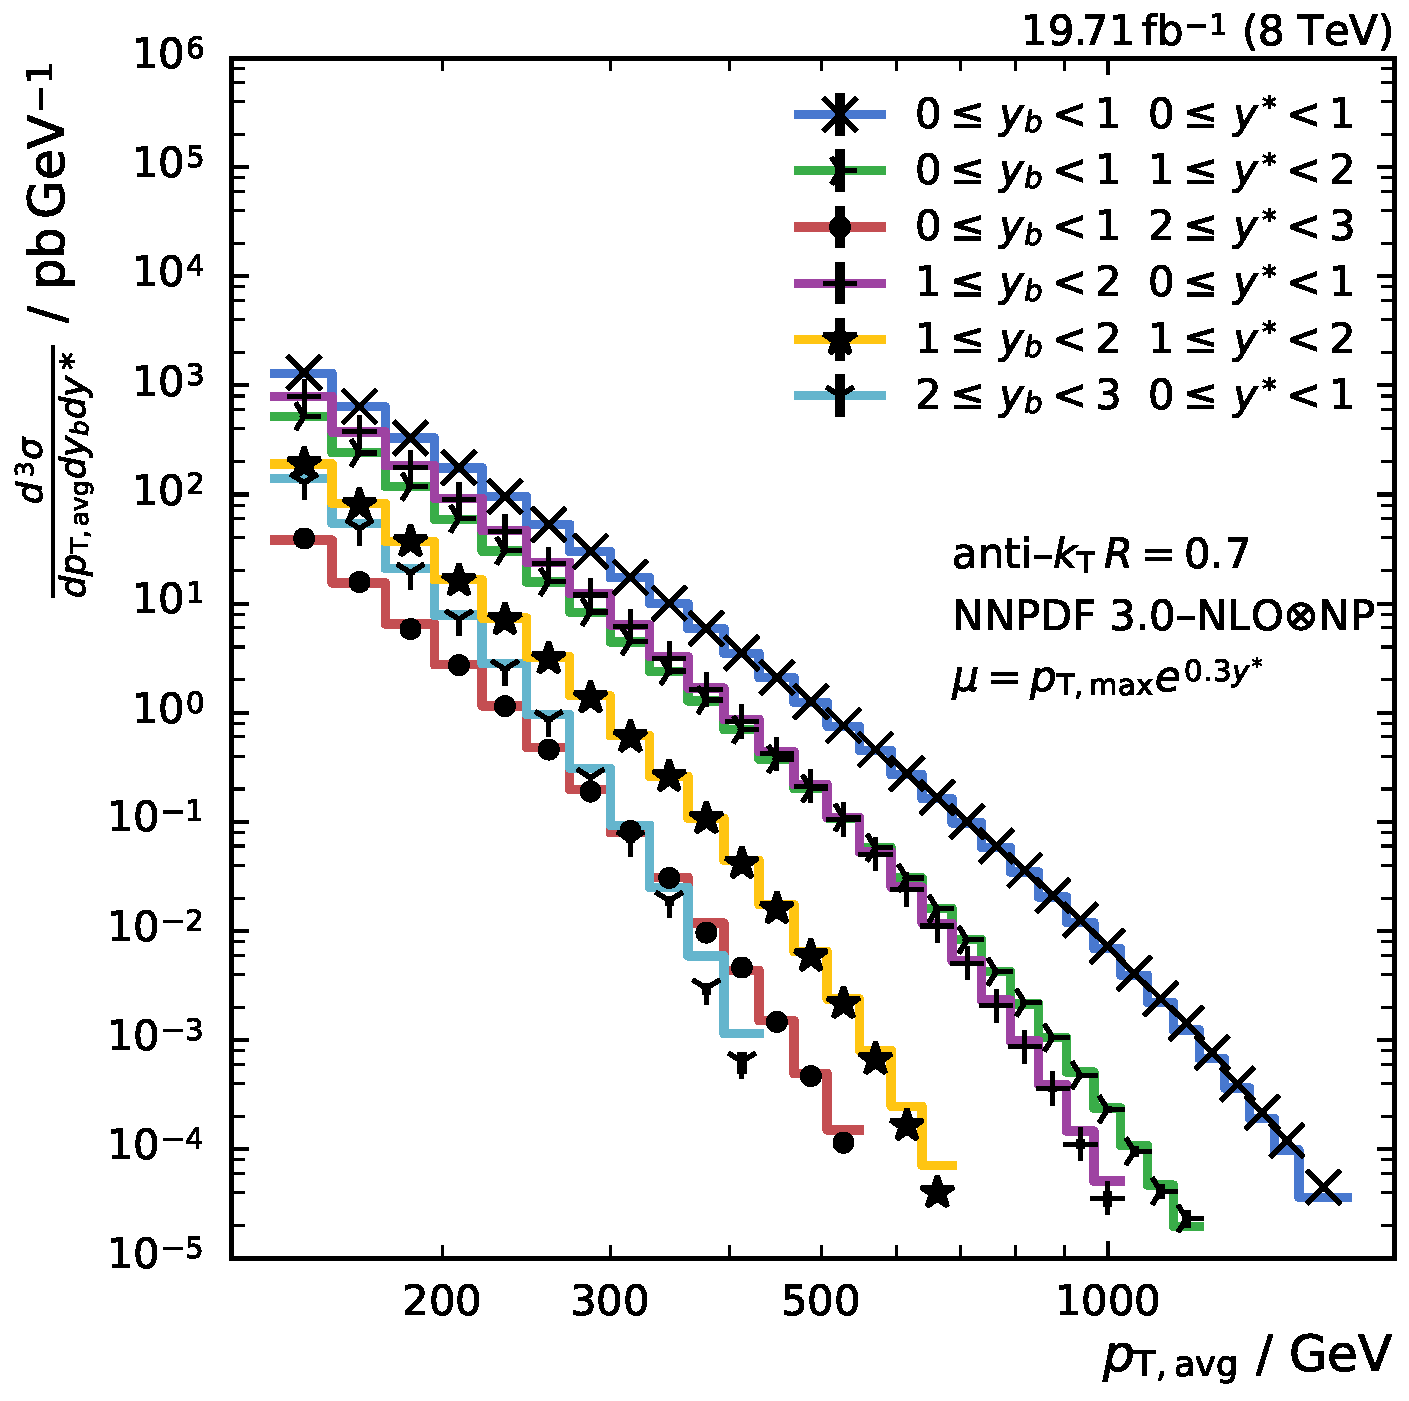
\includegraphics[width=0.45\textwidth]{figures/measurement/ptavg_spectrum.pdf}\hfill
    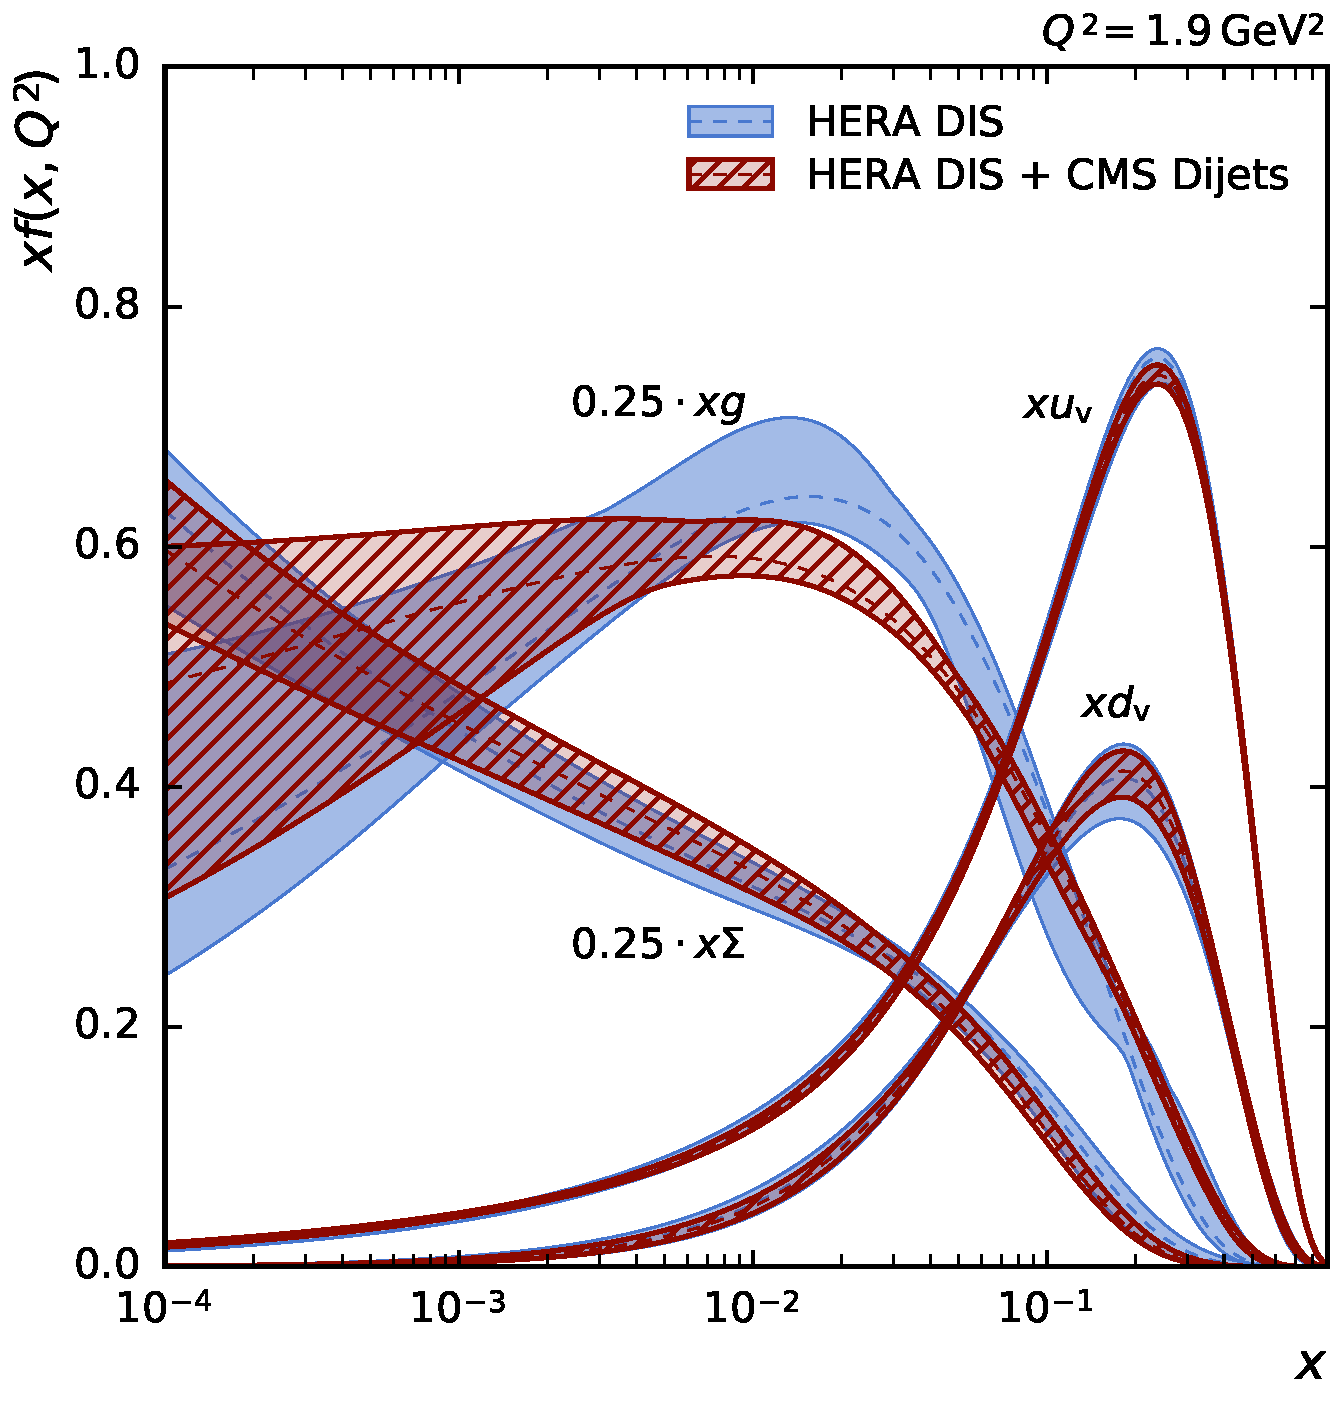
\includegraphics[width=0.45\textwidth]{figures/pdf_constraints/pdfcomp_direct_overview_1.9.pdf}
    \caption[Triple-differential dijet cross sections and PDF
    overview]{Left:
    The triple-differential dijet cross sections. The data points are indicated by black
    markers, the NLO theory prediction by colored lines. Right: Overview of
    fitted PDFs with and without including the triple-differential dijet
    measurement.}
    \label{fig:conclusion}
\end{figure}

Theoretical predictions have been calculated in pQCD at NLO accuracy and
corrected for non-perturbative effects. Fig.~\ref{fig:conclusion} left shows the
cross sections in the six studied \ystar and \yboost bins. It was found that the
data is well described by the predictions over many orders of magnitude. In
phase space regions containing boosted highly boosted dijet events, the data
discriminate between the predictions using different global PDF sets.

The small experimental uncertainties provide constraints on the proton PDFs. To
demonstrate the sensitivity of the PDFs to the measured cross sections, a
combined PDF fit of the HERA DIS data and the dijet cross sections was performed. It
was found that the PDFs are improved when the dijet data are included and the
uncertainties of the PDFs, especially of the gluon PDF, have been significantly
reduced. Fig.~\ref{fig:conclusion} right demonstrates the PDF constraints.

The strong coupling constant \asmz was determined by performing a simultaneous
fit of the PDFs and the strong coupling. The extracted value reads as

\begin{equation*}
  \asmz = 0.1188_{-0.0015}^{+0.0015}(\mathrm{exp})_{-0.0002}^{+0.0004}(\mathrm{mod})_{-0.0005}^{+0.0003}(\mathrm{par})_{-0.0010}^{+0.0029}(\mathrm{scale})
\end{equation*}

which is in good agreement with the world average value of the PDG. The
uncertainties on \asmz are dominated by the scale uncertainties which will
improve with the availability of NNLO calculations.

The pioneering studies presented in this thesis prove that the triple-differential
measurement of dijet cross sections using the chosen observables are an optimal
approach to perform QCD precision studies using jets. As soon as CMS has
collected enough data at $\sqrt{s}=\SI{13}{\TeV}$ further constraints can be
achieved. 

% nnlo calculations
